\chapter{Dark matter interpretations of Run 1 searches for invisibly decaying Higgs bosons}
\label{chap:interp}
As well as combining the results of the \ac{VBF} searches with other channels, it is also possible to interpret them as limits on models incorporating \ac{DM}. The particular models that are studied fall into two classes, \ac{EFT}s and simplified models, which are described in detail in \SectionRef{sec:DMextensions}. These studies were not carried out as part of the CMS collaboration, so it was necessary to develop and validate a framework for simulating the events resulting from these models.

%??CHECK PLOT AXIS LABEL SIZES AND THAT LEGEND TERMS ARE STANDARD OR IN TEXT

\section{Simulation Techniques and Validation}
\label{sec:dmval}
The CMS \textsc{Geant} based detector simulation is very computing intensive, so an alternative detector simulation with the \textsc{Delphes} fast reconstruction package was used. Whilst \textsc{Delphes} has been extensively validated by its authors against the CMS reconstruction~\cite{Favereau2014}, two of the variables used in the invisible Higgs boson decay searches described in this thesis are not implemented in the standard version of \textsc{Delphes}. Specifically, a calculation of the \MET ignoring objects with $|\eta>3|$ was added, to replicate the behaviour of the CMS \ac{L1} trigger. The total transverse energy calculated using all particles in the event with no minimum threshold on their energy, which is required for the calculation of \METsig, was also added.

Another difference from the CMS analysis is that the studies described in this chapter use \textsc{MadGraph} to simulate the hard-scattering process, whilst the CMS analysis uses \textsc{Powheg}. Both the internal CMS simulation and that described in this chapter use \textsc{Pythia} for parton-showering and hadronisation. Yields and kinematic distributions of events after selection criteria are applied are obtained from these simulations using an analysis framework developed and validated by the MasterCode collaboration~\cite{deVries:2015hva}.

%start with internal sample validate against \textsc{Powheg} plus delphes: when generated with same PU etc. found to agree to within 10% phenoplots281015.pdf
The validation of these simulations and the analysis framework was carried out in two steps, both using a centre of mass energy of 8 \TeV. First, \textsc{Powheg} and \textsc{Pythia} were used to simulate a \ac{VBF} produced 125 \GeV Higgs boson decaying to invisible final states, as in the internal CMS simulation. This sample of events is then processed using the \textsc{Delphes} based reconstruction and MasterCode analysis framework. The resulting event yields are compared to those obtained from a \textsc{Powheg} and \textsc{Pythia} produced sample processed using the full CMS reconstruction and analysis framework. The event yields were found to agree within 10\%.


The second step was to compare the 125 \GeV \ac{VBF} produced invisibly decaying Higgs boson sample generated with \textsc{Powheg} to one generated with \textsc{MadGraph} with both samples being processed using \textsc{Delphes}. This comparison was carried out starting from the following requirements:
\begin{align}
  \label{eq:dmvalstart}
  \begin{split}
\eta_{j1}\cdot\eta_{j2}<0, \rm{jet\,1\,and\,jet\,2\,}\pt>35 \GeV, \METsig>3,\\ \detajj>3.6, \Mjj>700 \GeV, \rm{L1} \MET>40 \GeV.
  \end{split}
\end{align}
Cuts were then added to this selection one at a time until the applied selection was the same as the parked data analysis signal region selection, which is listed in \EquationRef{eq:parkedsigsel}. The resulting event yields can be seen in \TableRef{tab:mgvsPowhegdelphes}. It is important to note that the \textsc{MadGraph} samples include both \ac{VBF} and \ac{VH} production of the Higgs boson, while the \textsc{Powheg} samples only include \ac{VBF} production. This difference explains the \textsc{MadGraph} yield being larger than that from \textsc{Powheg} at the starting point of the comparison. As the selection is tightened the disagreement between \textsc{Powheg} and \textsc{MadGraph} can be seen to reduce until the difference in yield is below 5\% for the full selection, where very few \ac{VH} events are still present. Only event yields after the full selection are used in the results presented in \SectionRef{sec:dmresults}, so the level of agreement is considered good.
%agreement can be seen to be good, the madgraph+delphes sim then used to generate samples at several mass points and for all the efts, met and eta for representative subsample of these shown in fig

%validate 	extsc{Powheg} plus delphes against mg plus delphes table from phenoplots281015.pdf
\begin{table}
  \caption{Event yields obtained, for several sets of event selection requirements, from two samples where the hard-scatter was simulated using \textsc{MadGraph} (second column) and \textsc{Powheg} (third column), both of which were processed using the \textsc{Delphes} fast detector reconstruction package. For each line the selection stated in the first column is added to the selection present for the line before. The starting point for the selection is described in \EquationRef{eq:dmvalstart}.}
  \label{tab:mgvsPowhegdelphes}
  \begin{tabular}{lcc}
    \hline
    \hline
    Selection added & \textsc{MadGraph} & \textsc{Powheg} \\
    \hline
    Start point & 2653 & 2311 \\
    jet 1 $p_{T}>50$ GeV, jet 2 $p_{T}>45$ GeV & 2056 & 1834 \\
    \METnoMU$>90$ GeV & 2000 & 1793 \\
    \Mjj$>1200$ GeV & 704 & 689 \\
    \METsig$>4$ & 539 & 519 \\
    \jetmetdphi$>2.3$ & 244 & 248 \\
    \hline
    \hline
  \end{tabular}
\end{table}

%limit validation to show no effect of correlations
The Run 1 signal and background estimates made public in \ReferenceRef{CMS-PAS-HIG-14-038} are quoted with their statistical and systematic errors. However, no information on the correlation between the signal and background systematic errors is given. In order to estimate the effect of these correlations the limits obtained, the observed and expected limits for the Run 1 parked data \ac{VBF} Higgs to invisible search were calculated assuming no correlation between the signal and background uncertainties. The observed (expected) 95\% \ac{CL} limit on \BRinv for a 125 \GeV Higgs boson was found to be  0.58 (0.42), which agrees well with the 0.57 (0.40) obtained using the full CMS uncertainty model. Correlations between the signal and background uncertainties were therefore considered negligible.

Having validated the simulation and uncertainty models at Run 1's 8 \TeV centre of mass energy, projections of the expected performance of the analysis at the increased 13 TeV Run 2 centre of mass energy were made. The validated \textsc{MadGraph} hard-scattering plus \textsc{Delphes} detector reconstruction simulation framework was used to generate events from the signal models described in \SectionRef{sec:DMextensions} at a centre of mass energy of 13 \TeV. The distribution of \MET for a representative sample of these models is shown in \FigureRef{fig:dmmodelkinematics}. It can be seen that whilst all of these models result in large values of \MET compared to the selection present in the \ac{VBF} Higgs to invisible searches, the \MET is typically less than 500 \GeV. The assumption that the momentum transferred through the mediator is less than the mediator's mass, that must be made in the case of the \ac{EFT} models, is therefore valid for mediators with masses above 500 \GeV.

\begin{figure}
  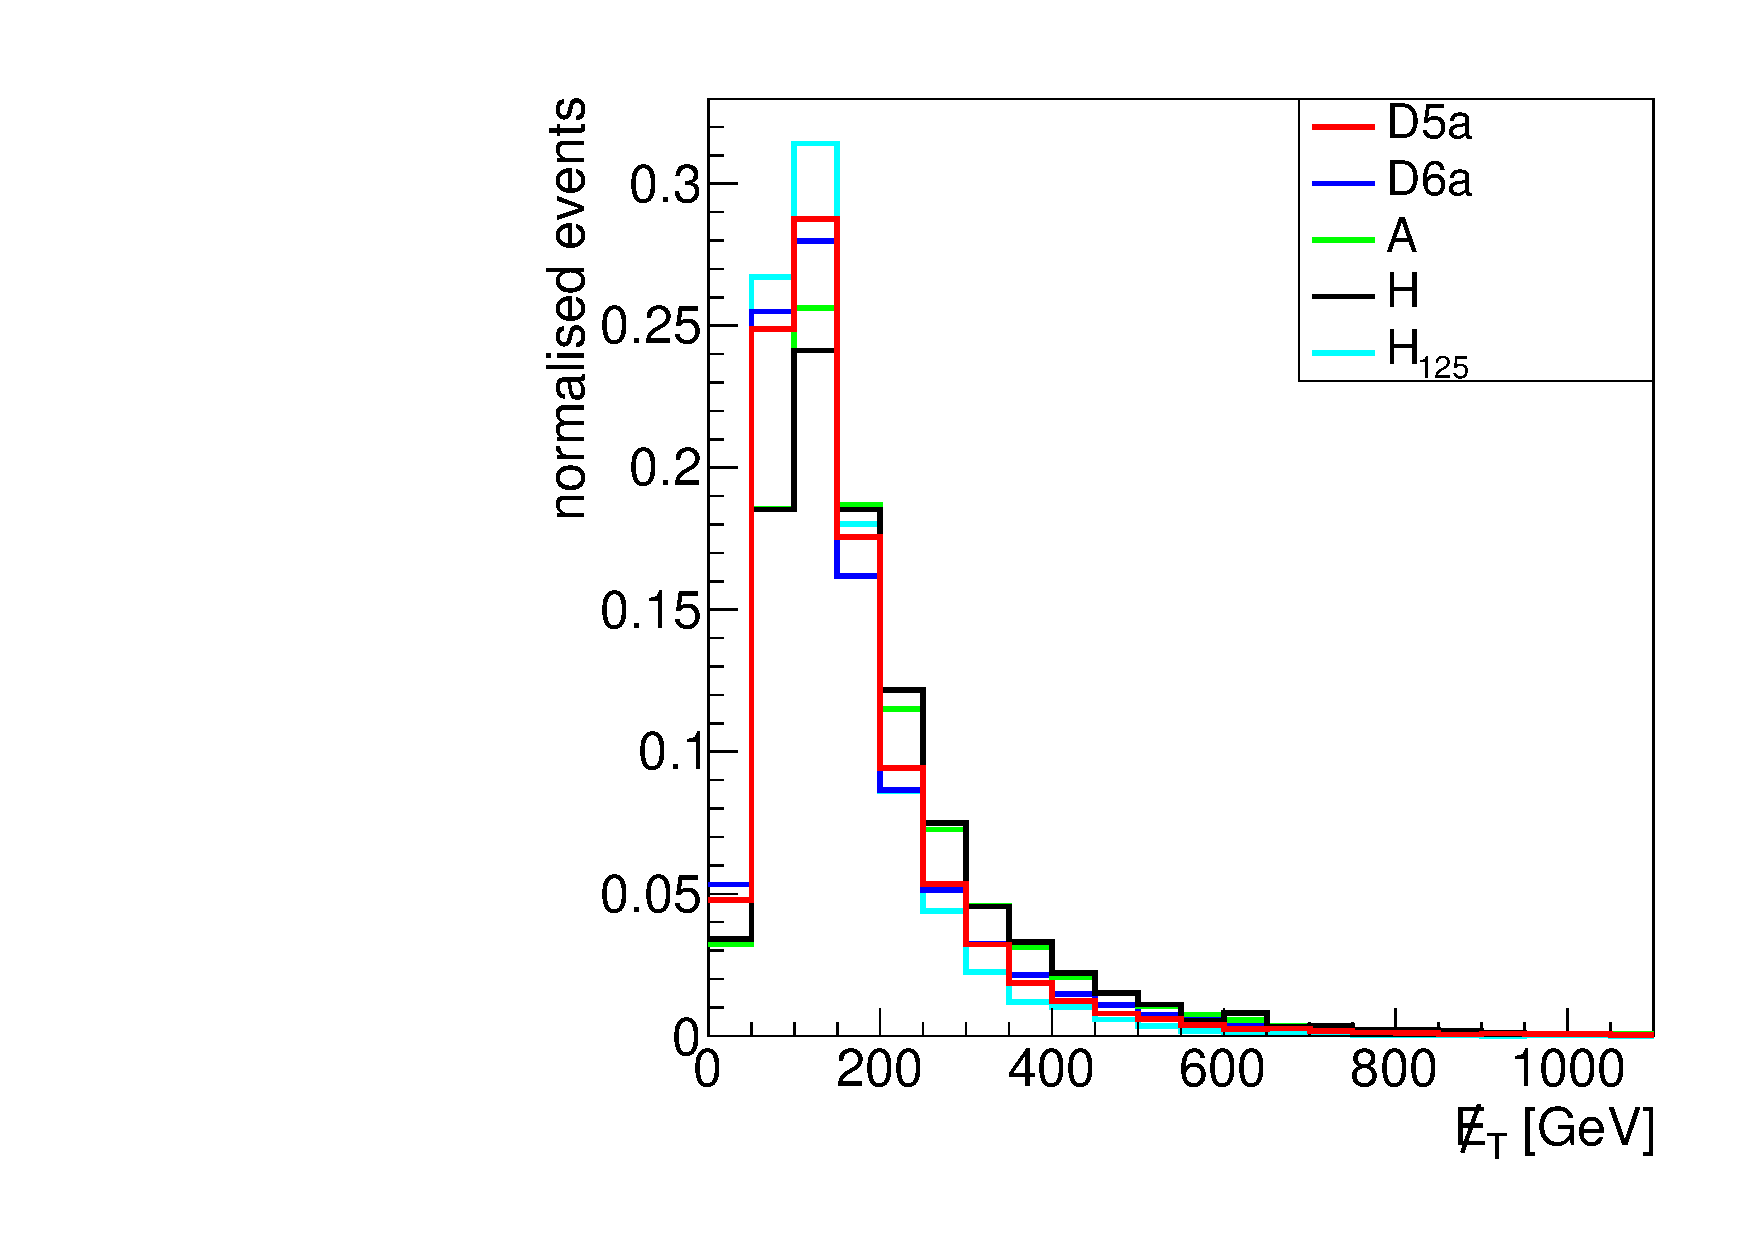
\includegraphics[width=\largefigwidth]{plots/interp/modelmet.pdf}
  \caption{The \MET distribution for two \ac{EFT} signal models (D5a and D6a), and spin-0 simplified models, described in \SectionRef{sec:DMextensions}, with representative model parameter values. For the \ac{EFT}s, heavier scalar (H) and pseudoscalar (A) models the dark matter mass, $m_{\chi}$ is assumed to be 100 \GeV, whereas for the 125 \GeV Higgs boson model $m_{\chi}$ is assumed to be 56.2 \GeV. For the scalar and pseudoscalar models the mass of the mediator is assumed to be 316.2 \GeV. It is important to note that the 125 \GeV Higgs boson model simulation includes \ac{VH} production of the Higgs boson as well as \ac{VBF}~\cite{ourdmpaper}.}
  \label{fig:dmmodelkinematics}
\end{figure}

%background scaling
In order to carry out estimations of the sensitivity of \ac{VBF} Higgs to invisible searches using the Run 2 LHC data, it is also necessary to estimate how the yield expected from background processes changes when the centre of mass energy is increased. The yields expected from each background process at 8 \TeV, listed in \TableRef{tab:parkedresults}, were therefore scaled by the cross-section ratio between 13 and 8 \TeV. These cross-section ratios were calculated using \textsc{Fewz} 3.1 for \PW and \PZ boson production, \textsc{Top++} v2.0 for top quark pair production and \textsc{MadGraph} for diboson production. Samples of \PW and \PZ bosons produced in association with jets were also produced at centre of mass energies of 8 and 13 \TeV, using the same simulation framework used for the signal processes. The efficiency for these events to pass the full Run 1 parked data \ac{VBF} Higgs to invisible search selection was then calculated. The expected yields from \PW and \PZ boson plus jets backgrounds, which make up 94\% of the background events expected, were corrected using the ratio between this selection efficiency obtained at 8 and 13 \TeV. The resulting total expected yield from background processes is 741 events.

%systematic scaling
In addition to scaling the expected event yields, the uncertainties on the yields must also be calculated. When extrapolating from 8 to 13 \TeV all statistical uncertainties are scaled by the square root of the ratio between the expected yield at 8 \TeV to the expected yield at 13 \TeV. The statistical uncertainties are then assumed to scale with the square root of the integrated luminosity collected at 13 \TeV.

For the systematic uncertainties, for 19.2 \invfb of integrated luminosity collected, the Run 2 fractional systematic uncertainties are assumed to be the same as those seen in the Run 1 parked data analysis. Two prescriptions are then used to estimate how the systematic uncertainties change with the integrated luminosity. The first prescription is to keep the systematic uncertainties constant as the integrated luminosity changes. The second, more realistic, prescription is to assume that the fractional systematic uncertainty scales as $1/\sqrt{\mathcal{L}}$, as many systematic uncertainties result from measurements which use statistically limited data samples. This second prescription also implies that for integrated luminosities below 19.2 \invfb\,the fractional systematic uncertainty will be larger than that seen in the Run 1 parked data \ac{VBF} Higgs to invisible search.


\section{Results}
\label{sec:dmresults}
%first project 125 GeV higgs limits on and off-shell
First, the sensitivity of the CMS search for invisibly decaying 125 \GeV Higgs bosons was projected to 13 \TeV for several integrated luminosities. The results of this projection are shown in \FigureRef{fig:smprojectedlimits}a for both systematic uncertainty scaling prescriptions. It can be seen that assuming the systematic uncertainties improve with square root of the integrated luminosity, CMS has the potential to exclude values of \BRinv as small as $\sim 5\%$. However, this will require control of systematic uncertainties at the 1\% level. Assuming the systematic uncertainties do not improve, the sensitivity of the analysis becomes systematically limited when $\sim 100$ \invfb\, of integrated luminosity have been collected, at  a limit on \BRinv of approximately 20\%. Given that the assumption that the systematic uncertainties show no improvement with increasing luminosity is very conservative, the rest of the results in this chapter assume the second, square root of integrated luminosity, uncertainty scaling prescription.

The next projection made was for the limit that can be obtained on the coupling of \ac{DM} to the 125 \GeV Higgs boson, $g_{\chi}$. For on-shell Higgs bosons this projection was made using \EquationRef{eq:offshellsmhiggs}, whereas for off-shell Higgs bosons, the assumption of equal couplings to visible particles and \ac{DM} was made and the \ac{DM} production rate was calculated as described in \SectionRef{sec:DMextensions}. The results of this projection are shown in \FigureRef{fig:smprojectedlimits}b, for integrated luminosities of 20, 300, and 3000 \invfb, which are those expected to be collected by CMS by the end of 2016, Run 2 and the high luminosity upgrade of the LHC respectively. It can be seen that whilst the limits on $g_{\chi}$ are considerably weaker for off-shell production, values of the coupling of order 1 can still be excluded with 3000 \invfb.

\begin{figure}
  \subfloat[]{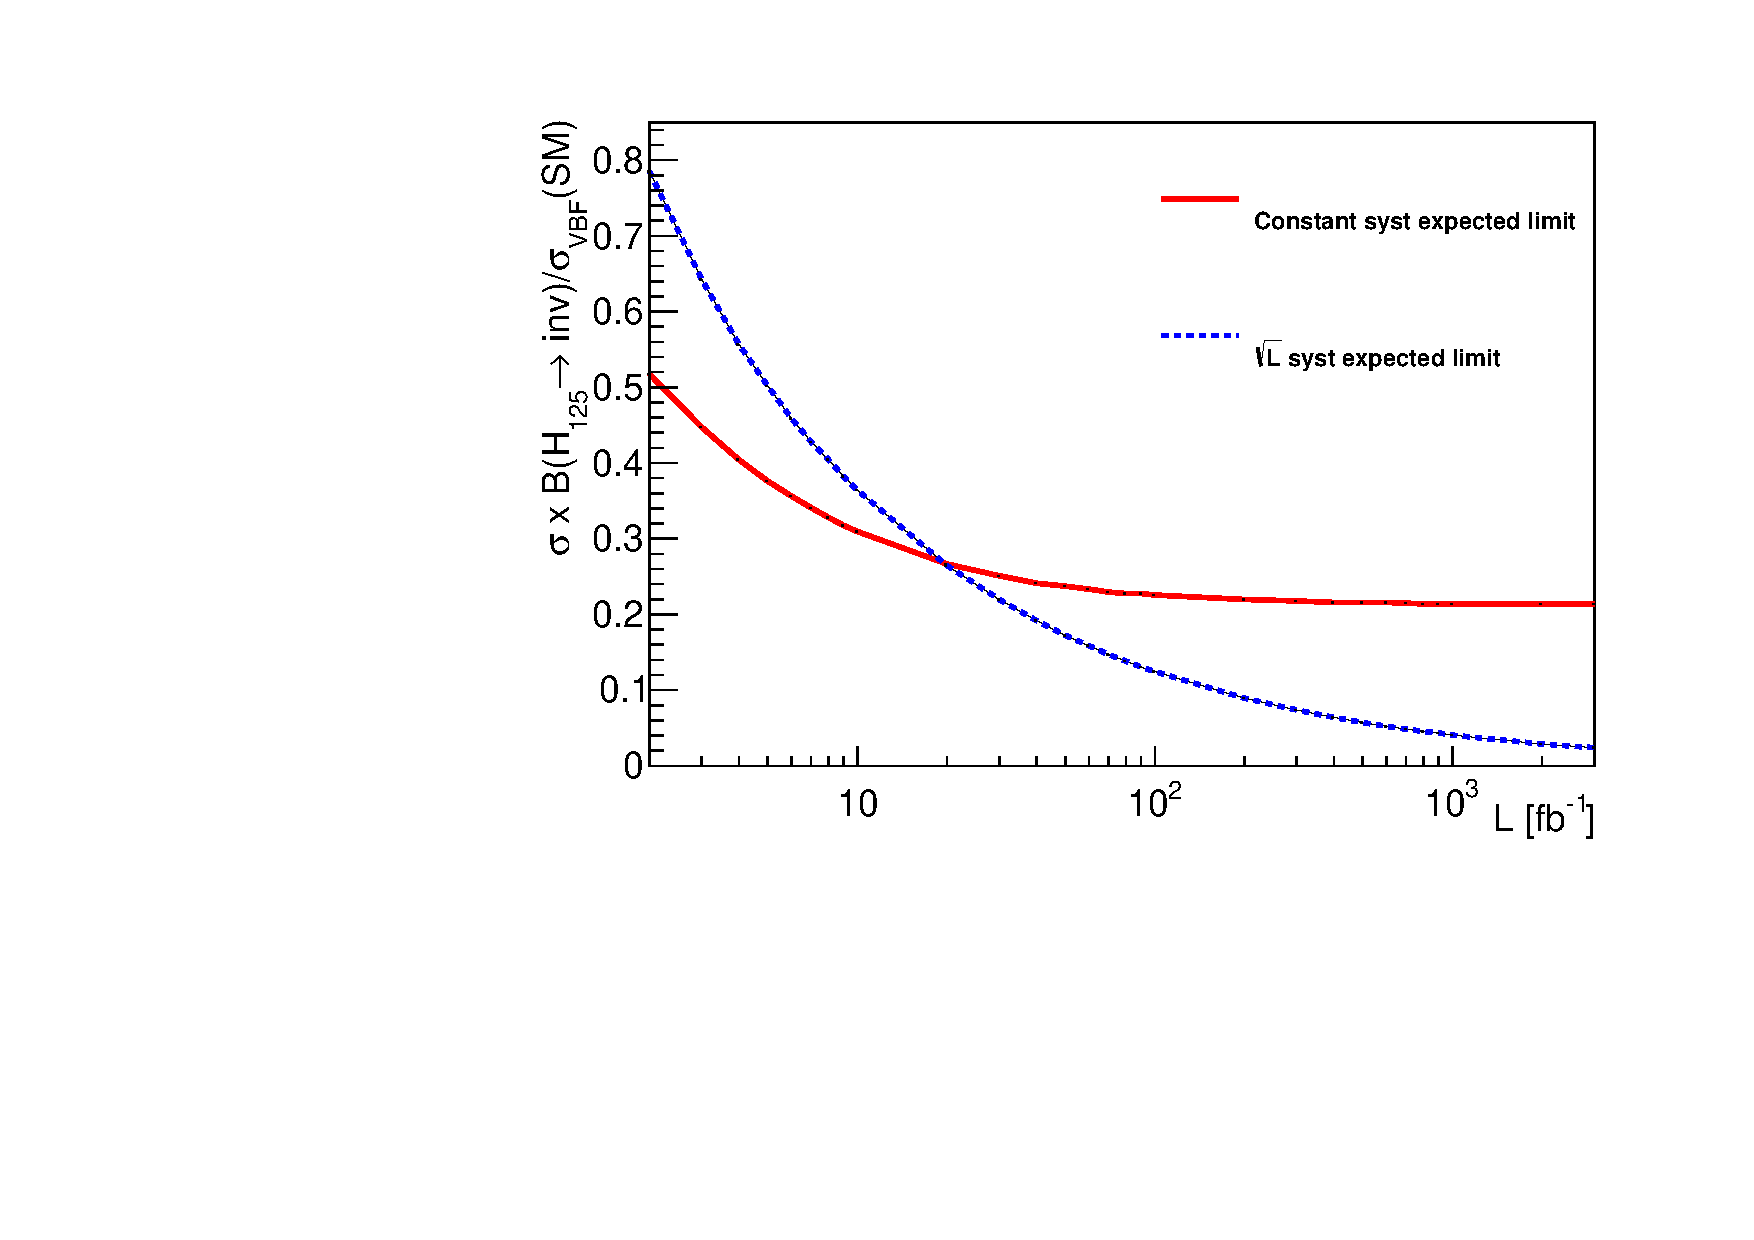
\includegraphics[width=\largefigwidth]{plots/interp/phenoprojectedvbflimit.pdf}}

  \subfloat[]{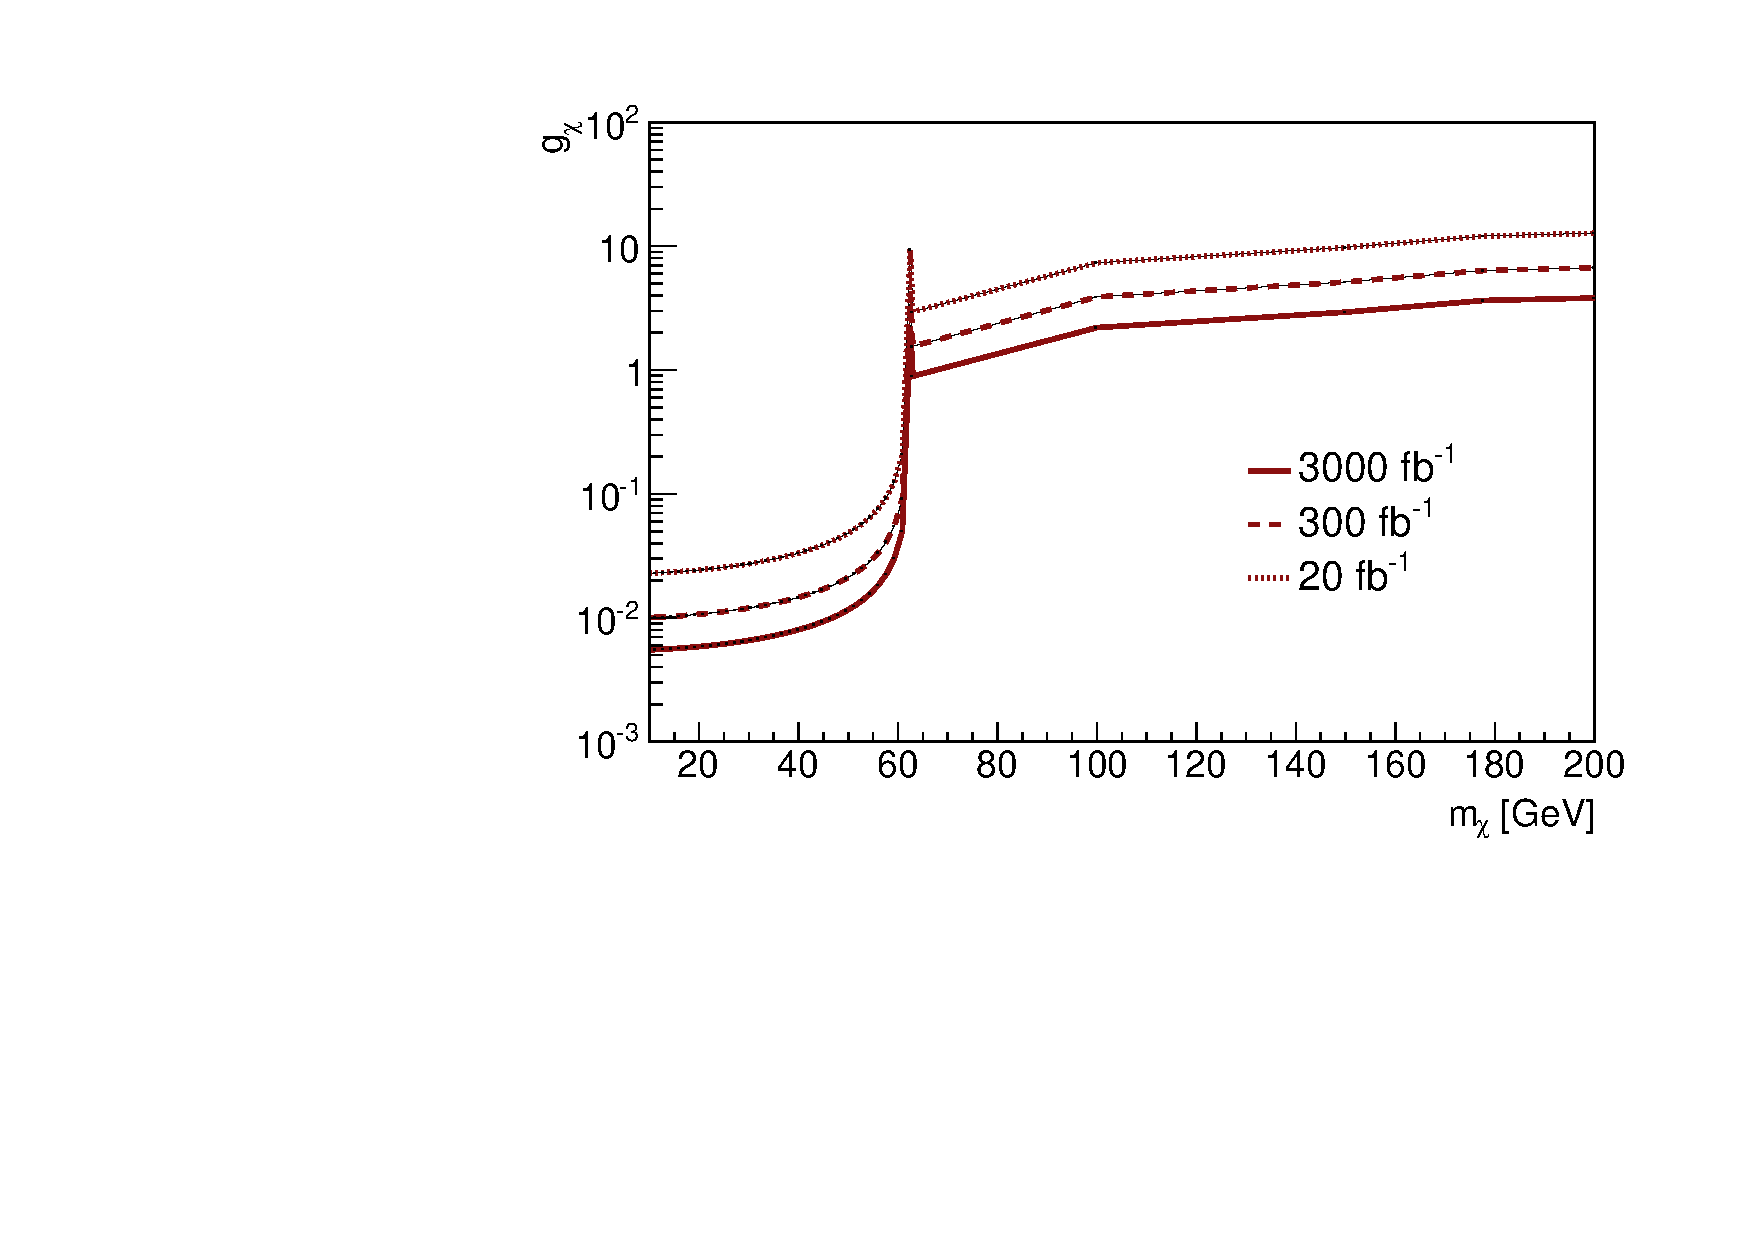
\includegraphics[width=\largefigwidth]{plots/interp/125higgsgchilimit.pdf}}
  \caption{(a) Expected limits on \BRinv for a 125 \GeV Higgs boson, as a function of integrated luminosity, projections were made both assuming constant systematic uncertainties (red) and assuming the systematic uncertainties improve with the square root of the integrated luminosity (blue). (b) Expected limits on the coupling of \ac{DM} to the 125 \GeV Higgs boson, $g_{\chi}$, as a function of \ac{DM} mass, $m_{\chi}$ for several integrated luminosities ~\cite{ourdmpaper}.}
  \label{fig:smprojectedlimits}
\end{figure}

%non 125 GeV simplified models
Next, projections were made of the limits on the couplings of spin 0 mediators with non-125 \GeV masses to \ac{DM}. As described in \SectionRef{sec:DMextensions} for \ac{DM} production via an on-shell mediator, the rate of production is proportional to $g_{\chi}^{2}$, whereas for production via off-shell mediators it is proportional to $g_{v}^{2}g_{\chi}^{2}=g_{\chi}^{4}$. This difference leads to a discontinuity in the projected limits at the on-shell to off-shell boundary. The projected limits obtained on scalar and pseudoscalar mediators are shown in Figures ~\ref{fig:simplifiedmodellimits}a and ~\ref{fig:simplifiedmodellimits}b respectively as a function of mediator and \ac{DM} mass for both the on and off-shell production regions. Very large luminosities are required to exclude values of the coupling of order $\pi$ or below due to the production rates for these models being very low. However, for large couplings \ac{DM} and mediator masses up to 1 \TeV can be excluded.

\begin{figure}
  \subfloat[]{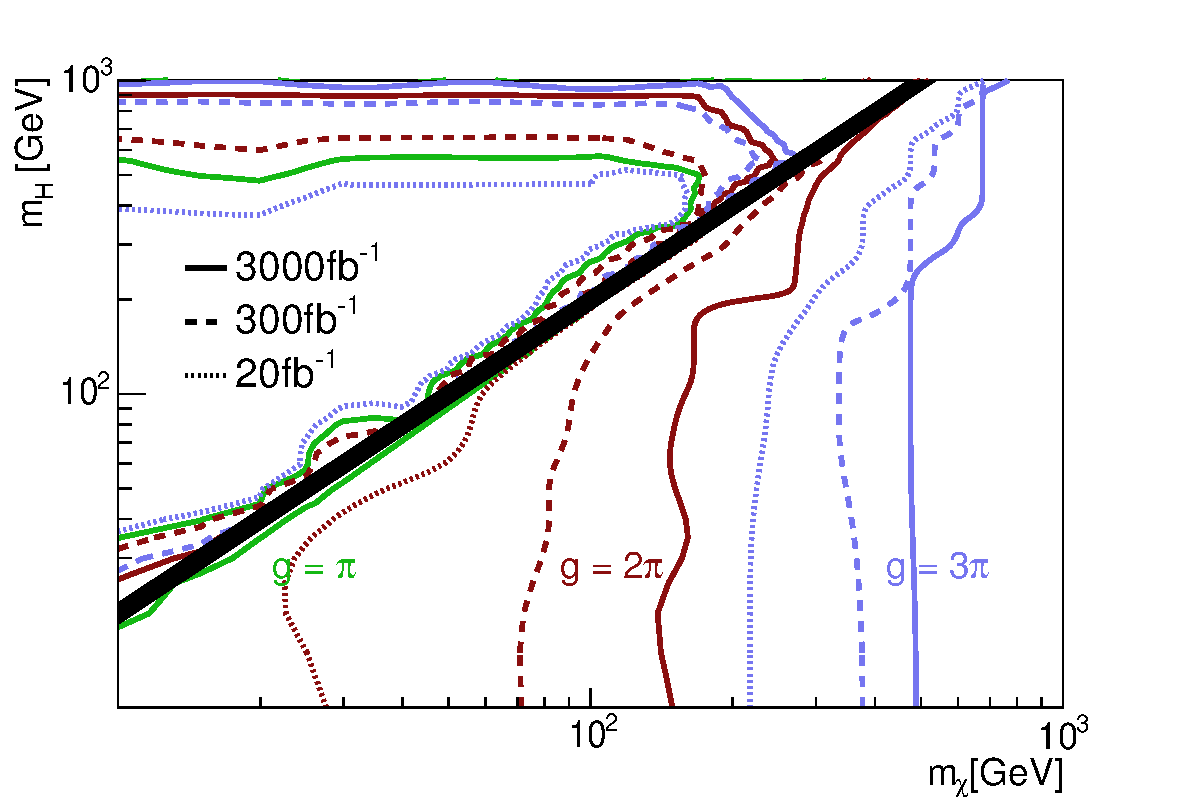
\includegraphics[width=\largefigwidth]{plots/interp/Hplane.pdf}}

  \subfloat[]{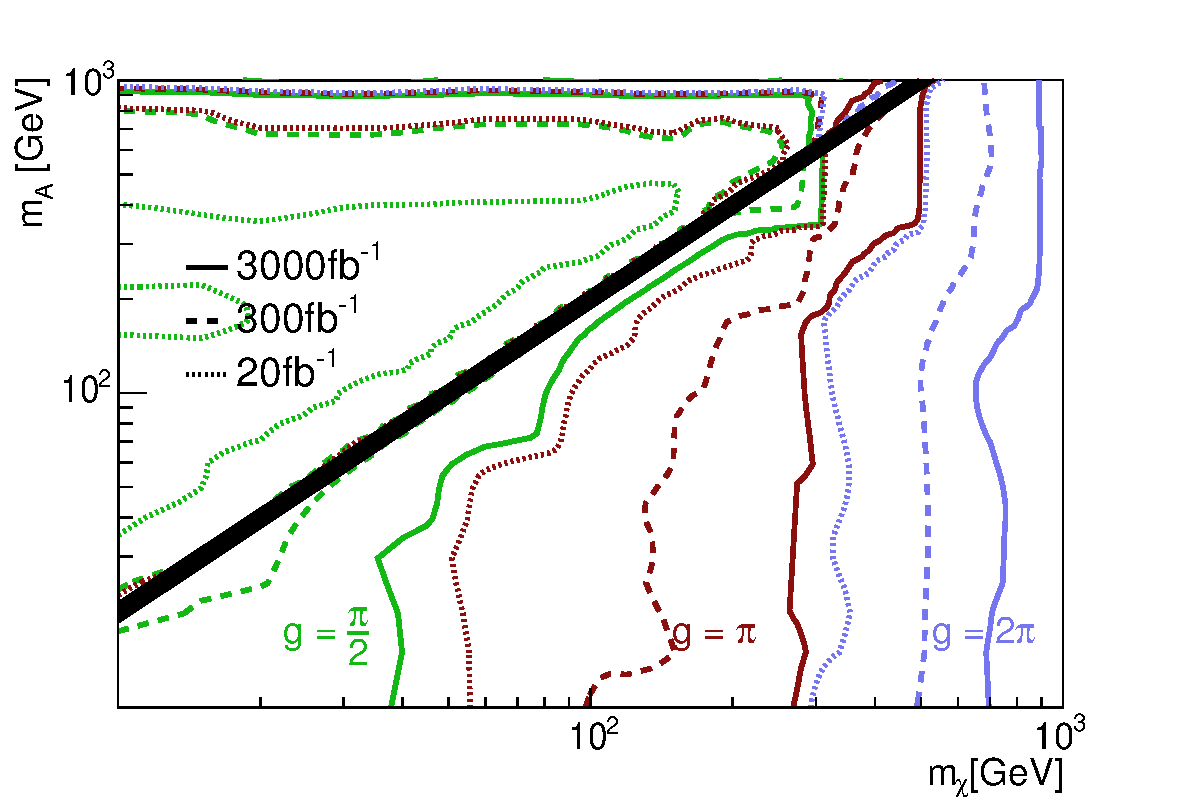
\includegraphics[width=\largefigwidth]{plots/interp/Aplane.pdf}}
  \caption{Expected exclusions on the coupling of \ac{DM} to scalar (a) and pseudoscalar (b) mediators as a function of mediator mass, $m_{H}/m_{A}$, and \ac{DM} mass, $m_{\chi}$. Note that some contours are not shown because the corresponding value of the coupling is not excluded at that integrated luminosity~\cite{ourdmpaper}.}
  \label{fig:simplifiedmodellimits}
\end{figure}

%efts
Finally, limits are set on the \ac{EFT} class of models. Limits on the D5, D6 and D7 operators are shown in Figures \ref{fig:eftlimits}a, \ref{fig:eftlimits}b and \ref{fig:eftlimits}c respectively. Several of the \ac{EFT}s produce very similar limits, so a subset has been chosen for clarity. It is important to note that the values of $\Lambda$ that are probed are much higher than the approximately 500 \GeV average momentum transfer expected through the mediator, as shown in \FigureRef{fig:dmmodelkinematics}, justifying the \ac{EFT} assumptions made, for couplings of order 1 or below.

As the power of $\Lambda$ by which the coupling to \ac{DM} is suppressed increases with the dimensionality of the operator, it would be expected that the D5 models would have the most sensitivity, with the D6 and D7 models being less sensitive. Whilst the D5a model does provide the best sensitivity, with values of $\Lambda$ up to 5 \TeV being excluded with the full LHC dataset, it can be seen from \FigureRef{fig:eftlimits} that there are several deviations from this pattern. The D5c and D5d operators exclude significantly lower values of $\Lambda$ than D5a and D5b, due to the primary \ac{DM} production mechanism being via a single \PZ boson (as can be seen from Equations 1.23 and 1.24) resulting in a lack of forward jets. This production via a \PZ boson also explains the decrease in the limit on $\Lambda$ seen above $m_{\chi}=m_{\PZ}/2$.

Furthermore, the D6 and D7 operators show similar exclusions on $\Lambda$, despite the dimensionality being greater for the D7 models. This is again due to the lack of forward jets in the D6 operators which, like the D5c and D5d operators, allow \ac{DM} production through a single \PZ boson, while the D7 models don't.

\begin{figure}
  \subfloat[]{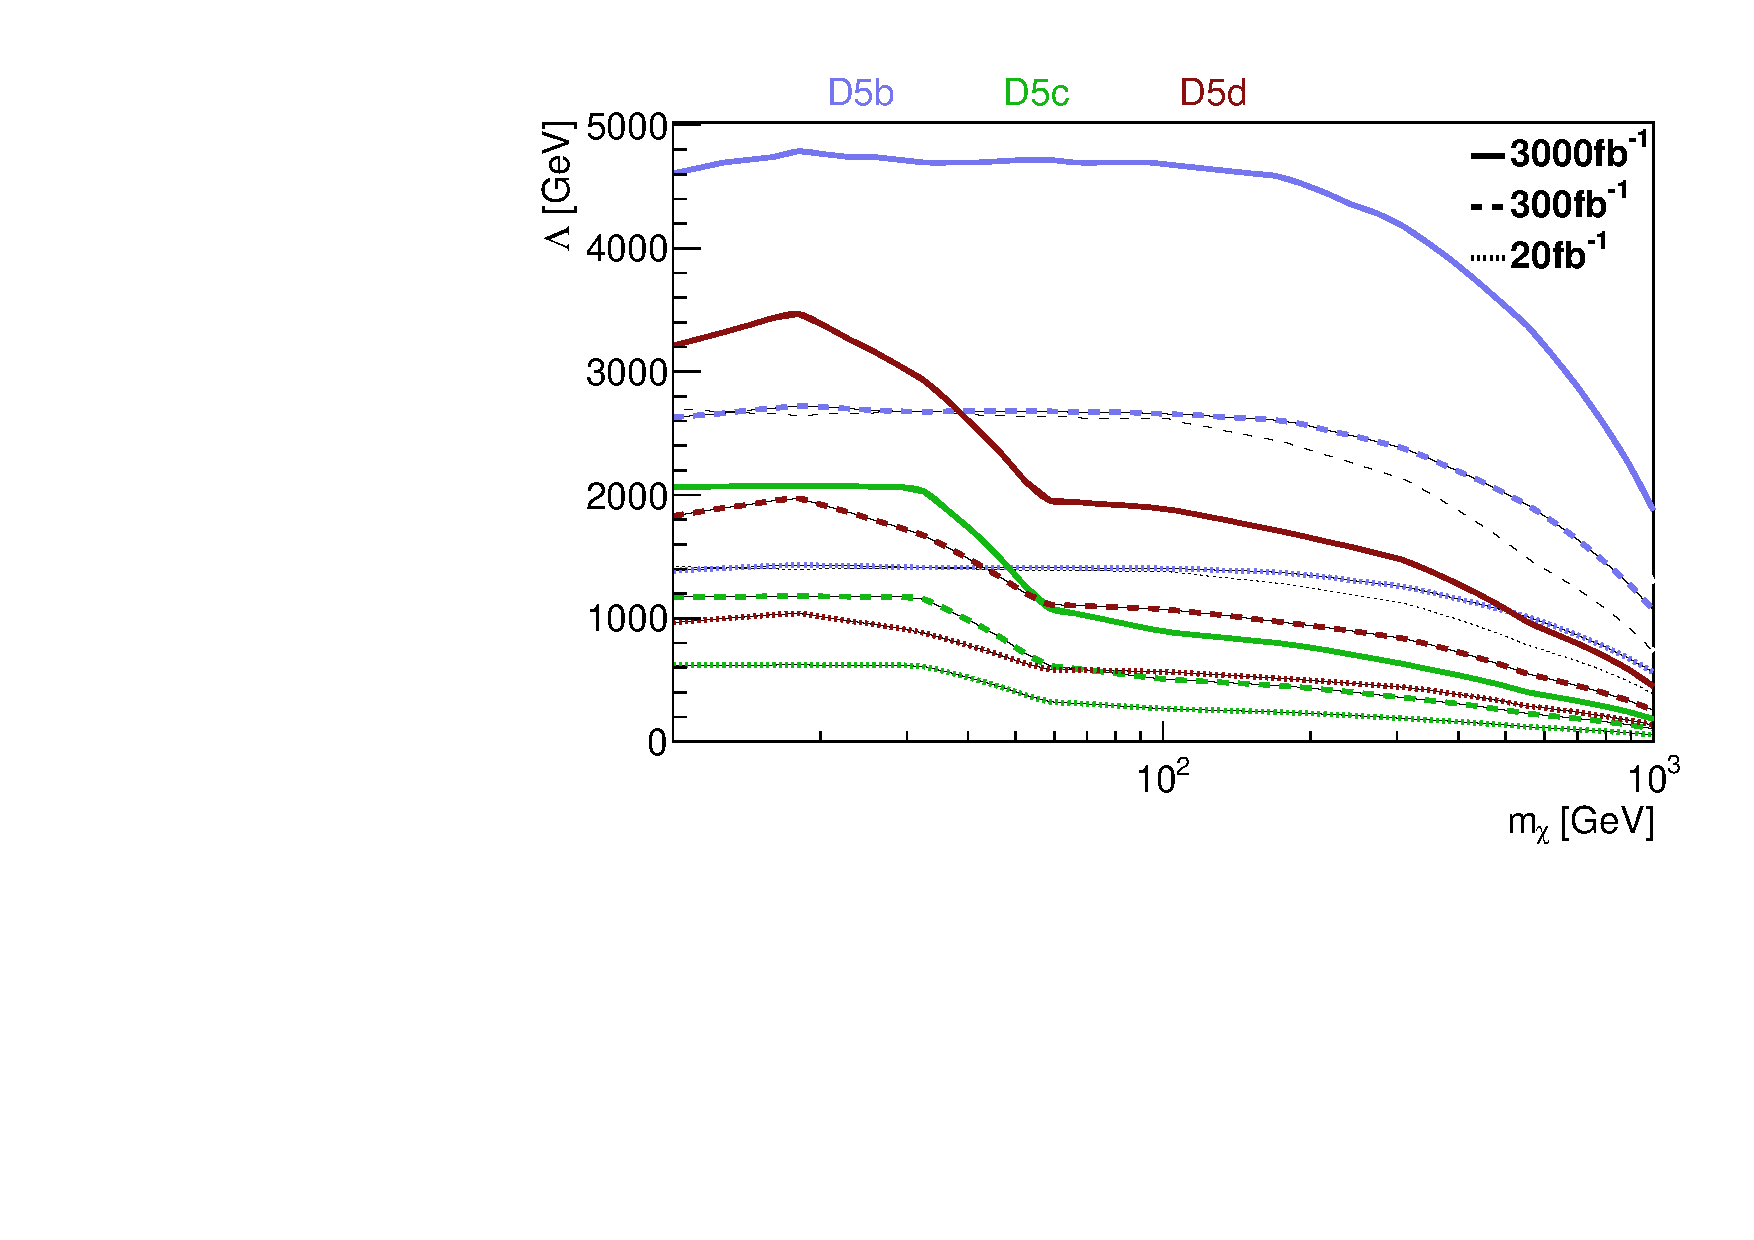
\includegraphics[width=.8\largefigwidth]{plots/interp/D5_multilumi.pdf}}

  \subfloat[]{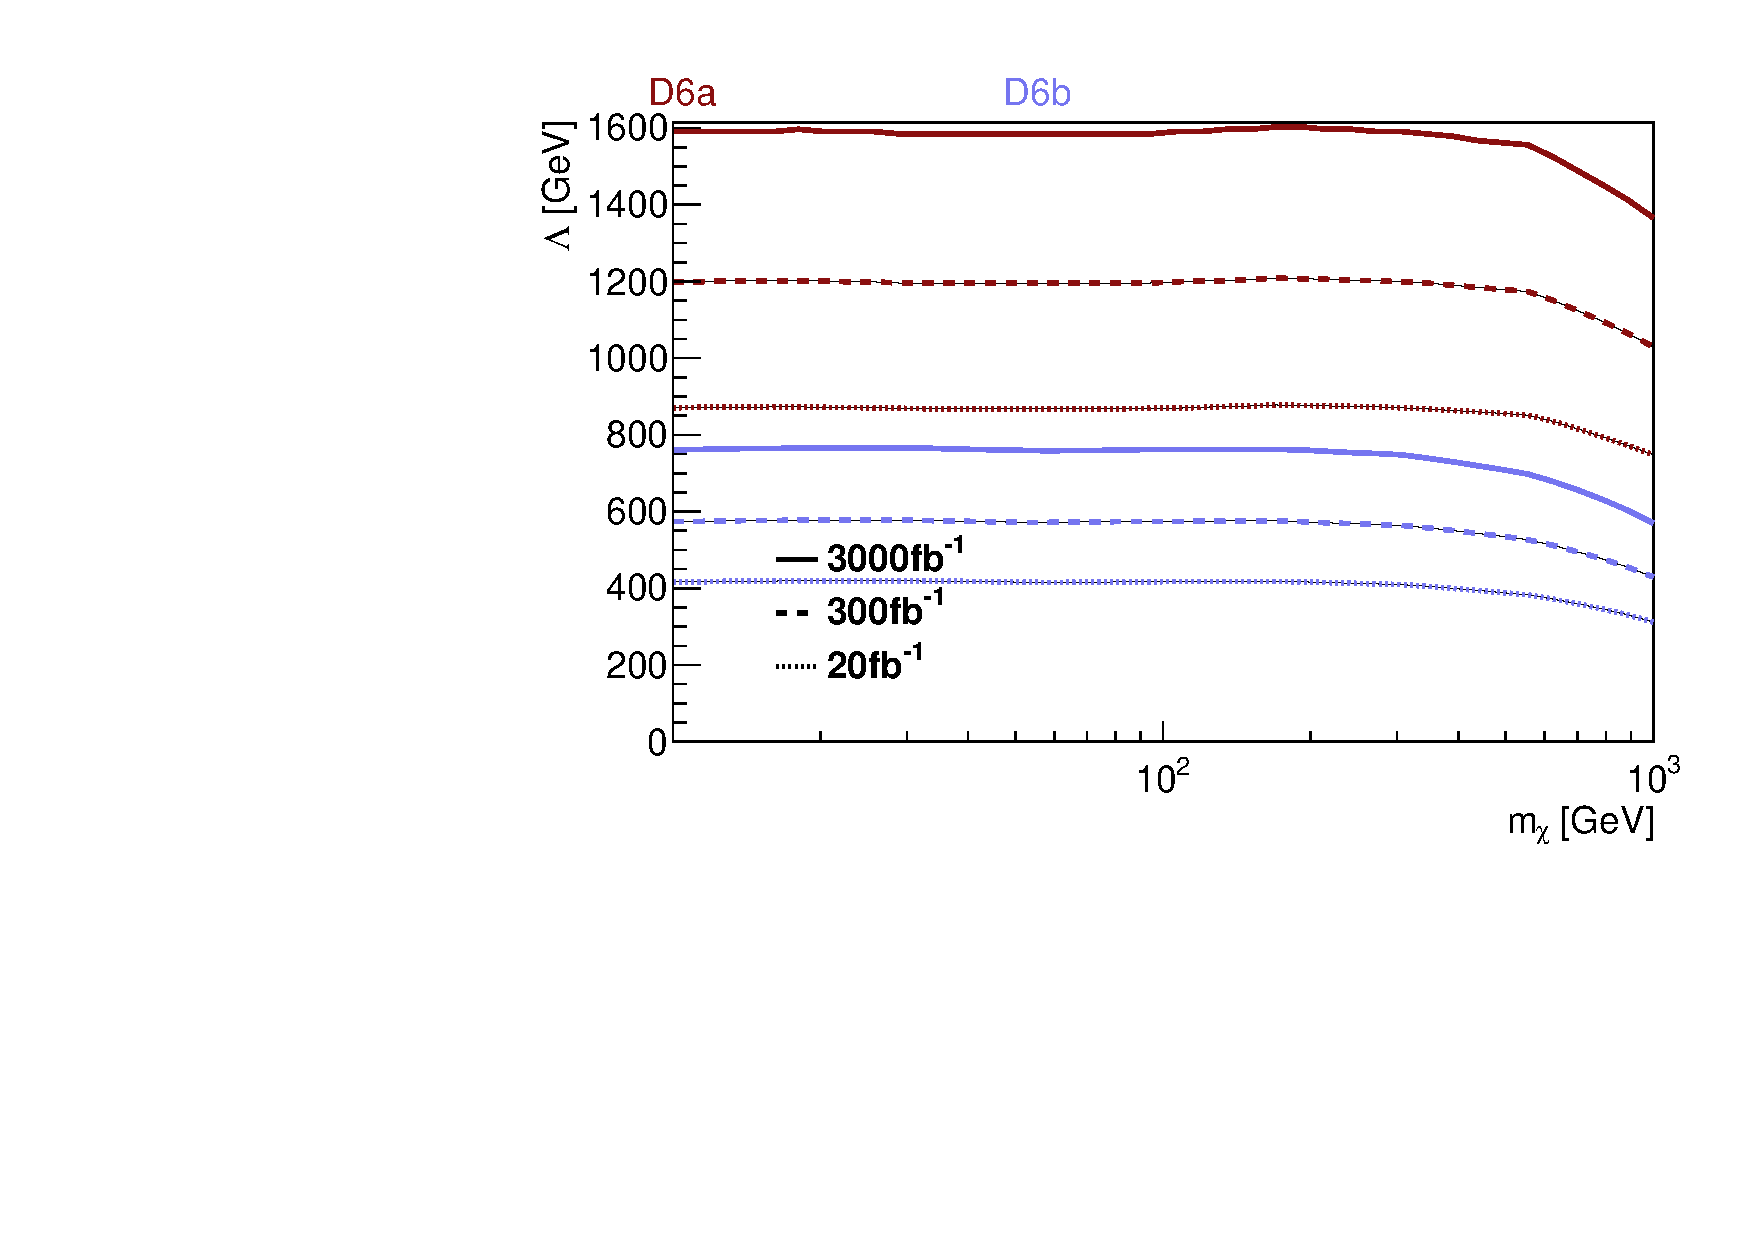
\includegraphics[width=.8\largefigwidth]{plots/interp/D6_2models.pdf}}

  \subfloat[]{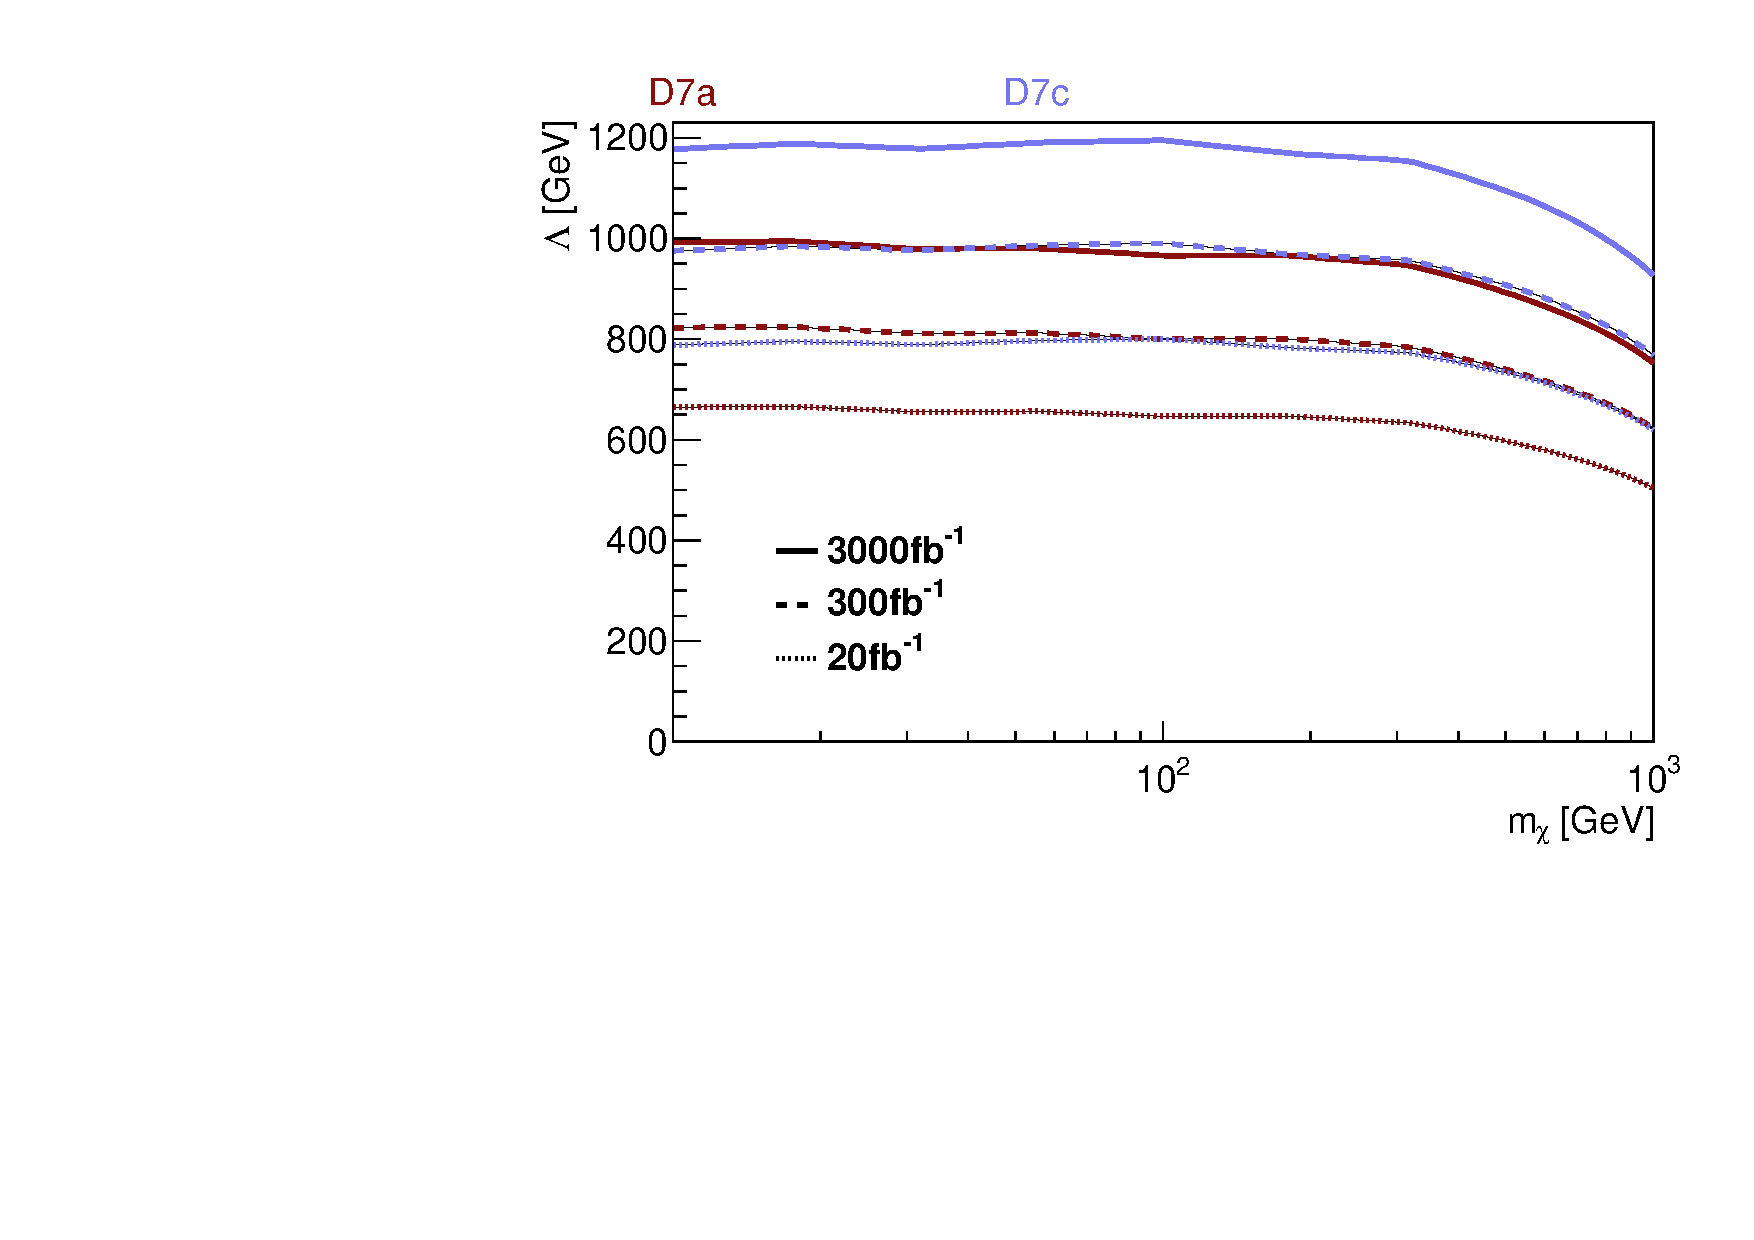
\includegraphics[width=.8\largefigwidth]{plots/interp/D7_2models.pdf}}
  \caption{Expected 95\% \ac{CL} lower limits on the \ac{EFT} scale, $\Lambda$, for D5 (a), D6 (b) and D7 (c) type \ac{EFT} operators for several values of the integrated luminosity. The D5a, D7b and D7d operators have very similar exclusions to the D5b, D7a and D7c operators respectively, so are not shown for clarity~\cite{ourdmpaper}.}
  \label{fig:eftlimits}
\end{figure}

\section{Conclusions}
\label{sec:dmconclusions}
%conclusion
In conclusion searches for invisible Higgs boson decays in the \ac{VBF} production channel in Run 2 will allow limits to be set on a wide range of models. The \ac{EFT} models studied will allow new physics to be probed up to the 5 \TeV scale in the case of the most sensitive operators. Simplified models with spin 0 mediators, large couplings, and mediator and \ac{DM} masses  up to the \TeV scale are also expected to be excluded by the end of LHC running. Furthermore, the direct limit on \BRinv for the 125 \GeV Higgs boson can be expected to reach 5\% after the full LHC dataset, providing systematic uncertainties improve with the square root of the integrated luminosity collected.
